\documentclass[10pt]{article}
\usepackage{graphicx}
% \usepackage{fullpage}
\usepackage{setspace}
\usepackage{natbib}
%%%%% \usepackage{lineno}
\usepackage[margin=3.2cm]{geometry}
\usepackage[singlelinecheck=off]{caption}
\usepackage{lineno}
\setcounter{secnumdepth}{-1}


\begin{document}
\title{Predator phylogenetic diversity decreases predation rate via
  antagonistic interactions} 
\author{A. Andrew M. MacDonald, Diane
  S. Srivastava, Gustavo Q. Romero}
%\date{November 2012}
\begin{spacing}{2}
\maketitle

\linenumbers

\section{Introduction}

\paragraph{Predators have important effects on ecosystems, and
  predator combinations could have either greater or smaller effects}
Predators play a critical role in many ecosystems; their presence can
have profound effects on community assembly \citep{Chase2009} and
enhance nutrient cycling \citep{Schmitz2010}.  Predator combinations
are known to have several possible outcomes -- predators may
interfere with each other, decreasing prey mortality, or may
compliment each other, causing an increase in prey mortality.  Such
changes in the strength of top-down control could affect both the
species composition and the function of the entire community.
However, few experiments have attempted to link predator-predator
interactions to whole community effects.

\paragraph{Predators may have both direct and indirect effects on each
  other and on lower trophic levels.} Predators may interact with each
other directly, or indirectly via the prey community.  Intraguild
predation among diverse predator assemblages is well known
(REF). Predators may also respond to each other's presence, by
altering feeding rate or foraging behaviour. Similarly, predators may
affect each other via their effects on prey.  Predators which consume
the same prey species will be in strong competition to each other,
while those selecting different prey will compete weakly.  Predators
may also affect prey behaviour via trait-mediated effects
\citep{Schmitz2007}. There are many possible indirect trait mediated
interactions between diverse predators: for example, diverse predator
combinations could have a stronger negative effect on prey behaviour
than either alone, resulting in a net decrease in predation.
Alternatively, prey avoidance of one predator may increase predation
by another, resulting in a net increase in predation. However
predators interact, their combined effect will change the
density and feeding rate of their prey, which in turn will affect
lower tropic levels (including the basal resource).  

\paragraph{predation rate affects ecosystem function} As predators
consume prey and/or alter the behaviour of that prey, the effects will
be felt throughout the food web.  Decreased prey density or feeding
rate will result in an increase in the standing crop of the next-lower
trophic level; these effects will therefore propagate down to all
trophic levels.  Theoretical work has demonstrated that the effect of
predation attenuates down the food chain, and that the ultimate
effects on the basal resource depend on the number of tropic links
(Loreau). In a meta-analysis of predator effects on 13 detritus-based
chains, \citet{Schmitz2007} suggested that food-chain length
determines the effect of predators on decomposition rates in
detritus-based food webs. The overall effects of predation on ecosystem
function will therefore depend on trophic structure. Previous work in
Costa Rican bromeliads has demonstrated that an increase in nutrient
cycling in bromeliads occurs when predators are present
\citep{Ngai2006}.  This may be caused by a decrease in successful
emergence by detritivores, a process that would otherwise remove
nitrogen from the system.

\paragraph{Despite studies of the effects of food chain length, we know little
about the complex effects of multiple predators at once.}%see
                                %meta-analyses: Cardinale et al
                                %(Nature)& Balvanera et al Ecol Lett
                                %(06 or 07) and A.Wilby's paper on
                                %multiple pred effects.
The effect of a diverse predator assemblage will depend on the
diversity of functional traits represented, including diet breadth,
feeding mode and habitat requirements
\citep{Schmitz2009}. \citet{Ives2005} suggest that predator-prey
interactions can lead to increased ecosystem function through niche
complementarity (e.g. different feeding modes, habitats or diet
breadths). \citet{Griffin2011} found that rates of predation increased
in strength and temporal stability in salt marshes when two species of
predatory crabs were present. \citet{Byrnes2006}, in a study in a
kelp-based food web, found that predators had an additional effect on
decreasing feeding by surviving herbivores; predator combinations
showed an additive increase.  Despite a large number of studies, we
still know little about how predator diversity might affect ecosystem
function.

\paragraph{If relevant traits are conserved within clades;
  phylogenetic diversity could be a useful predictor of predator
  functional diversity and ecosystem-level effects.} Phylogenetic
diversity gives us a robust and inclusive measure of diversity that
includes many possibly unmeasured traits, and therefore might predict
ecosystem function more closely than simply species richness
(Srivastava \emph{et al.}  in prep). For example, in a study by
\citet{Maherali2007}, diverse mycorrhizal communities had both higher
species richness and greater function (plant biomass) after a year,
due to complementarity between fungi with high phylogenetic
diversity. To our knowledge, similar experiments with animals have yet
to be done. There is tantalizing evidence that such manipulations
would reveal an important effect: for example, detritus processing
chains (facilitation among detritivores caused by each species
breaking the food source into sizes suitable for another
\citep{heard1994processing}) often include members of different
clades, since the feeding mode (and hence role within the processing
chain) varies more among than within higher-level taxonomic groups
\citep{Merritt2009}.

% While phylogenetic community ecology has made important progress in
% understanding the mechanisms of plant community diversity and
% function, work at higher trophic levels remains uncommon.
% Phylogenetic diversity of animals has recently become the subject of
% observational studies; \citet{Vamosi2009} survey 39 studies of
% phylogenetic community structure and report only 6 studies of animals
% (15\%).  Experiments which manipulate consumer phylogenetic diversity
% are even rarer. 

Non-additive effects of predator combinations may also increase with
PD. For example, intraguild predation results in decreased predator
density and a corresponding indirect effect on consumers. The
probability of intraguild predation may increase with phylogenetic
distance, since more dissimilar predators are more likely to be
different enough in body size and feeding mode that they are able to
successfully capture each other. Non-additive effects may also arise
if prey behaviour is altered by the presence of one predator in such a
way that the probability of capture by another species is enhanced or
decreased. For example, the threat of predaceous Plecoptera causes
stream insects to move to exposed rocks where they are easier prey for
fish \citep{Soluk1997}.

We attempted to measure the effects of predator combinations on
ecosystem function.  We approached this questions in three parts:
first, we quantified patterns of co-occurrence between predators, using
observational datasets.  Then, we attempted to measure diet breadth in
all species via a series of feeding trials.  Finally, we conducted a
community-level manipulation of predator phylogenetic diversity to
estimate its effects on prey emergence and ecosystem function.

\section{Methods}

% Introduction themes related to this: the presence/rarity of food web
% quantifications.  the large variation in ecosystem function (decomp
% rate) in bromeliads in this habitat (lecraw, unpub data).  does pred
% pd account for some of this? 


We combined predators together in species pairs that represented a
range of relatedness: congeners (two congeneric damselflies,
\emph{Leptagrion andromache} and \emph{Leptagrion elongatum}), two
insects (a damselfly, \emph{Leptagrion elongatum} and a predatory fly
(Diptera: Tabanidae)) and two invertebrates (\emph{L. elongatum} and
leeches).  We also included these four species in monoculture, along
with a predator-free control (8 treatments, n=5).  Combinations were
substitutive, maintaining the same amount of predator metabolic
capacity (biomass raised to the power of 0.69, predicting the scaling
of metabolism with body mass \citep{Brown2004}) in each.  Response
variables included the rate of decomposition of leaves, bromeliad
growth and insect emergence.  This experiment allows the estimation of
the effect of each predator species from monoculture treatments, as
well as the detection of non-additive effects in predator
combinations.

In Feburary 2011, bromeliads between 90 and 200ml were collected,
thoroughly washed and soaked for 12 hours in a tub of water.  They
were then hung for 48 hours to dry.  One bromeliad dissected after
this procedure contained no insects.

Each bromeliad was supplied with dried leaves, simulating natural
detritus inputs from the canopy.  We enriched these leaves with N-15
by fertilizing five (Jabuticaba, \emph{Genus species}) plants with
40ml/pot/day of 5g/L ammonium sulphate containing 10 percent atom
excess of N15. %%duration. started on 27/1/2011
Whole leaves were then picked from plants and air-dried until constant
weight, and then soaked for three days and the water discarded.  About
1.5 g of leaves were placed in each bromeliad.

Each bromeliad was stocked with a representative insect community.
The densities of each prey taxon were calculated from a 2008
observational dataset, using data from bromeliads of similar size to
those in our experiment (DS Srivastava, upub. data).  All densities
used were within the range of these calculated abundances, and all
experimental bromeliads received the same insect community.  Halfway
through the experiment, insects were added to bromeliads a second
time.

\begin{table}
  \centering
  \caption{densities of each species}
  \label{tab:sppden}
  \begin{tabular}{l l}
    \hline
    \emph{Chironomus detriticula} & 10 \\
    \emph{Polypedium} sp. 1 & 4 \\
    \emph{Polypedium} sp. 2 & 2 \\
    \emph{Psychodid} sp. 1 & 1 \\
    \emph{Scyrtes} sp. A & 5 \\
    \emph{Culex} spp. & 4 \\
    \emph{Trentepholia} sp. & 1
  \end{tabular}
\end{table}


% Densities were calculated from 2008 dataset survey in two ways: the
% first, by poisson regression and the second, by taking the average of
% all bromeliads in between 90 and 200ml (n = 6???). 

After addition of the prey community, all bromeliads were enclosed
with a mesh cage and checked daily for emergence of adults.

%% how much fine detritus was added?

%% exactly how much coarse was added?  mean and standard deviations
%% for each.

%% Exactly when was the second addition of the larvae?

%%%% must add in the hypotheses section from Proposal.tex - but not to
%%%% keep it as a bullet list!  or just keep in the specific
%%%% hypotheses tested?

\subsection{Analysis}
\label{sec:analy}

%% sections about the the analysis for the food web and co-occurance data

We tested our hypotheses about the effects of predator combinations by
comparing response variables of predator polycultures with the average
response of the two corresponding predator monocultures. Intraguild
predation should be visible in our experiment as different levels of
predator survival, while synergistic interactions among predators
would result in a higher prey mortality than in predator
monocultures. We used randomization tests to estimate the non-additive
effect of predator combinations.  In the presence of non-additive
effects, the effect of predator combinations should differ
significantly from the mean of the two monoculture treatments.  We
calculated this quantity by first calculating treatment means for each
experimental treatment.  Then, we averaged the two monoculture means
and subtracted this number from the corresponding polyculture mean.
We repeated this procedure for each pair of species represented in the
polyculture.

\section{Results}

Prey suvivorship varied among treatments, with the control showing the
highest emergence rate (number of surviving or emerging prey insects)
confirming that predator treatments reduced the successful emergence
of prey. Randomization tests confirmed that predator combinations had
more prey survivorship than monoculture treatments \ref{fig:prednonadd}.

%% would we see the same effects of predator survivorship?
\begin{figure}
  \centering
  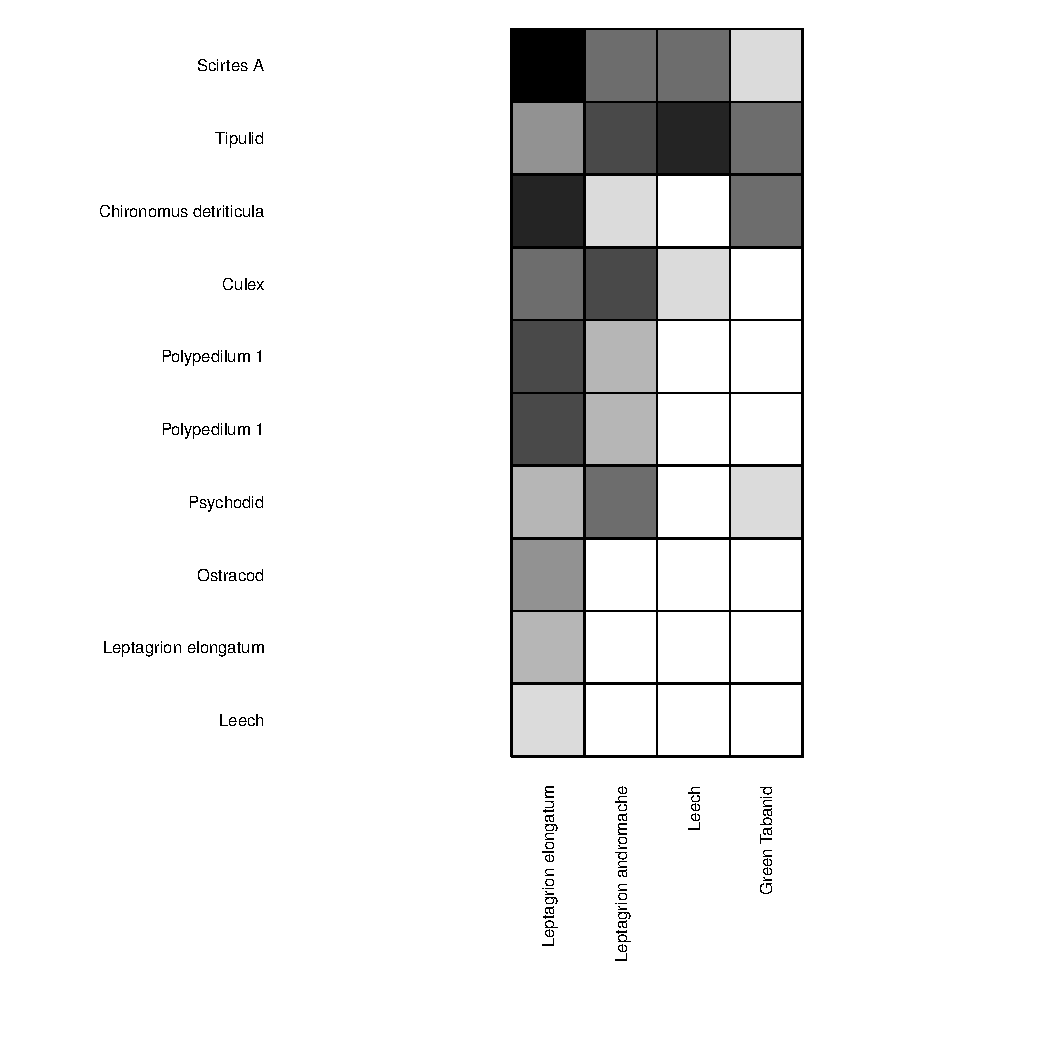
\includegraphics{../figures/foodwebVisweb.pdf}
  \caption{A diagram of the food web among the taxa used in this
experiment. The top row represents predators, and the bottom prey.
the width of the grey lines indicates the strength of predation. Data
is from controlled feeding trials in laboratory conditions.}
\label{fig:foodweb}
\end{figure}


\begin{figure}
  \centering
  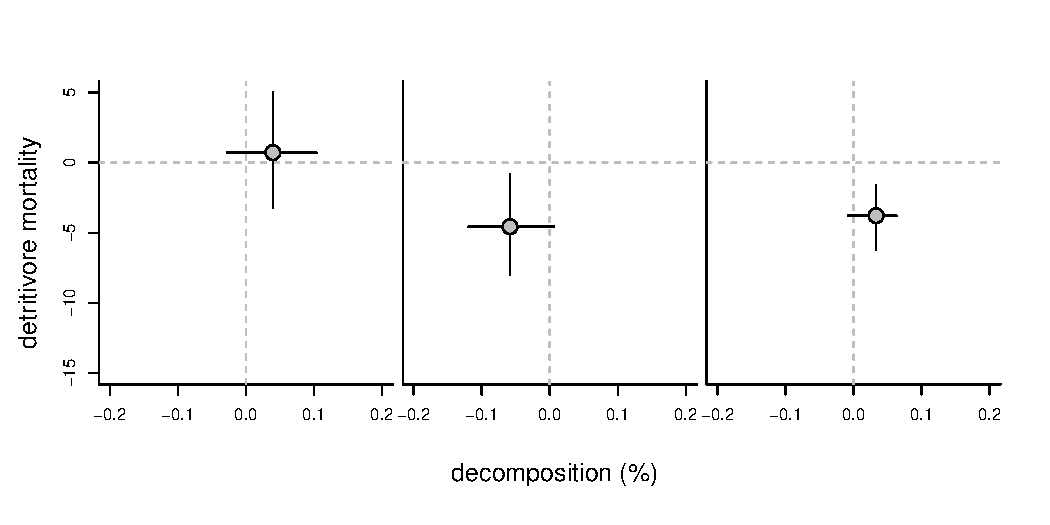
\includegraphics[width=0.9\textwidth]{../predator.div.experiment/bivar.pdf}
  \caption{The non-additive effects of predator combinations. Percent
    decomposition is the change in mass of the coarse detritus which
    was supplied in each bromeliad.  Survivorship is the sum of
    emerged adults and also those prey larvae which were found still
    alive at the end of the experiment.  The non-additive effect is
    calculated as the difference between the mean of the monoculture
    treatments and the mean of the polyculture treatment. Solid lines
    indicate 95\% bootstrap confidence intervals.}
\label{fig:prednonadd}
\end{figure}


\section{Discussion}

It seems that this food web is dominated by omnivory.  Also, that
damselflies are highly sensitive to the presence of other predators,
which both decreases damselfly survivorship and perhaps also predation
rate.  Other work in the similar Costa Rican bromeliad communities
demonstrates that damselflies will voluntarily leave if in physical
contact with dytiscid beetles (Edd and Trisha's work?).

\end{spacing}

\bibliographystyle{../../Writing/sysbio3} \bibliography{../references/references.bib}
\end{document}
